\documentclass{article}


\usepackage{arxiv}
%\usepackage{ebgaramond}
\usepackage{garamondx}
% \usepackage{CormorantGaramond}

\usepackage[utf8]{inputenc} % allow utf-8 input
\usepackage[T1]{fontenc}    % use 8-bit T1 fonts
\usepackage{hyperref}       % hyperlinks
\usepackage{url}            % simple URL typesetting
\usepackage{booktabs}       % professional-quality tables
\usepackage{amsfonts}       % blackboard math symbols
\usepackage{nicefrac}       % compact symbols for 1/2, etc.
\usepackage{microtype}      % microtypography
% \usepackage{lipsum}		% Can be removed after putting your text content
\usepackage{amsmath} 
\usepackage{amssymb}
\usepackage{graphicx}
\usepackage{epstopdf}
\usepackage{url}
\usepackage{setspace}
\usepackage{amsthm}
\usepackage{mathrsfs}
\usepackage{enumitem}
\usepackage{parskip}
\usepackage{IEEEtrantools}
\usepackage{mathtools}
\usepackage{tensor}
\usepackage{yfonts}
\usepackage{dsfont}

%%%%%%%%%%%%%%%%%%% Custom packages
\usepackage{braket}
\usepackage{todo}
\usepackage{xargs}                      % Use more than one optional parameter in a new commands
\usepackage{tikz}
\usepackage{tikz-cd}

%%%%%%%%%%%%%%%%%%


\usepackage{pgfplots}
\pgfplotsset{compat=1.15}

\usetikzlibrary{arrows}



\newtheorem{theorem}{Theorem}[section]
\newtheorem{lemma}[theorem]{Lemma}
\newtheorem*{lemma*}{Lemma}
\newtheorem{prop}[theorem]{Proposition}
\newtheorem{corollary}[theorem]{Corollary}
\newtheorem{defn}[theorem]{Definition\rm}
\newtheorem{conjecture}[theorem]{Conjecture}
\newtheorem{remark}{\it Remark\/}
\newtheorem{example}{Example}
\newtheorem{fact}{Fact}

\newcommand{\st}{\ensuremath{:}}% such that
\newcommand{\ie}{\emph{i.e.} }
\newcommand{\eg}{\emph{e.g.} }
\newcommand{\cf}{\emph{cf.} }
\newcommand{\ra}{\rightarrow}
\newcommand{\la}{\leftarrow}
\newcommand{\lra}{\longrightarrow}
\newcommand{\lla}{\longleftarrow}
\newcommand{\lbracket}{\left(}
\newcommand{\rbracket}{\right)}

\newcommand{\al}{\alpha}
\newcommand{\w}{\omega}
\newcommand{\W}{\Omega}
\newcommand{\m}{\mu}
\newcommand{\n}{\nu}
\newcommand{\e}{\epsilon}
\newcommand{\K}{K\"ahler }
\newcommand{\HK}{hyperk\"ahler }
\newcommand{\into}{\hookrightarrow}
\newcommand{\PP}{\mathbb{P}}
\newcommand{\RR}{\mathbb{R}}
\newcommand{\CC}{\mathbb{C}}
\newcommand{\QQ}{\mathbb{Q}}
\newcommand{\FF}{\mathbb{F}}
\newcommand{\ZZ}{\mathbb{Z}}
\newcommand{\NN}{\mathbb{N}}
\newcommand{\HH}{\mathbb{H}}
\newcommand{\vp}{\varphi}
\newcommand{\mcA}{\mathcal{A}}
\newcommand{\mcE}{\mathcal{E}}
\newcommand{\mcF}{\mathcal{F}}
\newcommand{\mcG}{\mathcal{G}}
\newcommand{\mcH}{\mathcal{H}}
\newcommand{\mcL}{\mathcal{L}}
\newcommand{\mcO}{\mathcal{O}}
\newcommand{\mfg}{\mathfrak{g}}
\newcommand{\mfh}{\mathfrak{h}}
\newcommand{\mft}{\mathfrak{t}}
\newcommand{\mc}[1]{\mathcal{#1}}
\newcommand{\mf}[1]{\mathfrak{#1}}

\newcommand{\sslash}{\mathbin{/\mkern-6mu/}}
\newcommand{\sssslash}{\mathbin{/\mkern-6mu/\mkern-6mu/\mkern-6mu/}}

\newcommand{\pbrackets}[1]{\left( #1 \right)}
\newcommand{\bbrackets}[1]{\left[ #1 \right]}
\newcommand{\norm}[1]{|#1|^{2}}

\newcommand{\dbar}{\bar{\partial}}
\newcommand{\mrr}{\mu_{\mathbb{R}}}
\newcommand{\mcc}{\mu_{\mathbb{C}}}
\newcommand{\prr}{\phi_{\mathbb{R}}}
\newcommand{\pcc}{\phi_{\mathbb{C}}}

\DeclareMathOperator{\Lie}{Lie}
\DeclareMathOperator{\Aut}{Aut}
\DeclareMathOperator{\Tr}{Tr}
\DeclareMathOperator{\Image}{Im}
\DeclareMathOperator{\Ad}{Ad}
\DeclareMathOperator{\Diff}{Diff}
\DeclareMathOperator{\Vect}{Vect}
\DeclareMathOperator{\Sympl}{Sympl}
\DeclareMathOperator{\Span}{Span}
\DeclareMathOperator{\ind}{ind}
\DeclareMathOperator{\Td}{Td}
\DeclareMathOperator{\Ch}{Ch}
\DeclareMathOperator{\Ind}{Ind}
\DeclareMathOperator{\pt}{pt}
\DeclareMathOperator{\rk}{rk}
\DeclareMathOperator{\coker}{coker}
\DeclareMathOperator{\Pf}{Pf}
\DeclareMathOperator{\Vol}{Vol}
\DeclareMathOperator{\Res}{Res}

\DeclareMathOperator{\GL}{GL}
\DeclareMathOperator{\SO}{SO}
\DeclareMathOperator{\UU}{U}

\newcommand\restr[2]{{% we make the whole thing an ordinary symbol
		\left.\kern-\nulldelimiterspace % automatically resize the bar with \right
		#1 % the function
		\vphantom{\big|} % pretend it's a little taller at normal size
		\right|_{#2} % this is the delimiter
}}

\title{Geometric Quantisation of Hypertoric Manifolds by Symplectic Cutting}

\date{}	% Here you can change the date presented in the paper title
%\date{} 					% Or removing it

%\author{
%  David S.~Hippocampus\thanks{Use footnote for providing further
%    information about author (webpage, alternative
%    address)---\emph{not} for acknowledging funding agencies.} \\
%  Department of Computer Science\\
%  Cranberry-Lemon University\\
%  Pittsburgh, PA 15213 \\
%  \texttt{hippo@cs.cranberry-lemon.edu} \\
%% examples of more authors
%   \And
% Elias D.~Striatum \\
%  Department of Electrical Engineering\\
%  Mount-Sheikh University\\
%  Santa Narimana, Levand \\
%  \texttt{stariate@ee.mount-sheikh.edu} \\
%% \AND
%% Coauthor \\
%% Affiliation \\
%% Address \\
%% \texttt{email} \\
%% \And
%% Coauthor \\
%% Affiliation \\
%% Address \\
%% \texttt{email} \\
%% \And
%% Coauthor \\
%% Affiliation \\
%% Address \\
%% \texttt{email} \\
%}

\begin{document}
	\maketitle
	
	\begin{abstract}
		Lorem ipsum.
	\end{abstract}
	
	\section{Introduction}
	
	Lorem ipsum.
	
	\section{Hyperk{\"a}hler Reduction and Hyperk{\"a}hler Analogues}
	
	\subsection{Introduction and Definitions}
	
	A \emph{\HK manifold} is a Riemannian manifold $(M,g)$ equipped with three orthogonal, parallel complex structures $J_{1}, J_{2}, J_{3}$, satisfying the usual quaternion relations. These three complex structures give rise to three symplectic forms
	$$
	\w_{1}(v,w) = g(J_{1}v,w),\quad \w_{2}(v,w) = (J_{2}v,w),\quad \w_{3}(v,w) = g(J_{3}v,w),
	$$
	so that each $(g,J_{i},w_{i})$ is in its own right a \K structure on $M$ for $i = 1,2,3$. The complex-valued two-form $\w_{2} + \sqrt{-1}\w_{3}$ is a closed, non-degenerate, and holomorphic two-form with respect to the complex structure $J_{1}$. Thus any \HK manifold can be considered as a \emph{holomorphic symplectic} manifold with complex structure $J_{1}$, real symplectic form $\w_{\RR} := \w_{1}$, and holomorphic symplectic form $\w_{\CC} := \w_{2} + \sqrt{-1}\w_{3}$.
	
	An action of a Lie group $G$ on a \HK manifold $M$ is called \emph{hyperhamiltonian} if it is hamiltonian with respect to $\w_{\RR}$, and holomorphic hamiltonian with respect to $\w_{\CC}$, with a $G$-equivariant moment map
	$$
	\mu_{HK} := \mu_{\RR} \oplus \mu_{\CC} \longrightarrow \mf{g}^{\ast} \oplus \mf{g}_{\CC}^{\ast}.
	$$
	The following theorem describes the \emph{\HK quotient} construction, which is the quaternionic analogue of a \K quotient:
	
	\begin{theorem}[\cite{HKLR87}]
		Let $M$ be a \HK manifold equipped with a hyperhamiltonian action of a compact Lie group $G$, with moment maps $\mu_{1}, \mu_{2}, \mu_{3}$. Suppose that $\xi = \xi_{\RR} \oplus \xi_{\CC}$ is a central regular value for $\mu_{HK}$, and that $G$ acts freely on $\mu_{HK}^{-1}(\xi)/G$. Then there is a unique \HK structure on the \HK quotient $\mf{M} = M\sssslash_{\xi}G := \mu_{HK}^{-1}(\xi)/G$, with associated symplectic and holomorphic symplectic forms $\w_{\RR}^{\xi}$ and $\w_{\CC}^{\xi}$, such that $\w_{\RR}^{\xi}$ and $\w_{\CC}^{\xi}$ pull-back to the restrictions of $\w_{\RR}$ and $\w_{\CC}$ on $\mu_{HK}^{-1}(\xi)$.
	\end{theorem}
	In general, the action of $G$ on $\mu_{HK}^{-1}(\xi)$ will not be free, but only locally free. In this situation, we would end up with a \emph{\HK orbifold}. However in the sequel, we shall only concern ourselves when the action is free, and that $\mf{M}$ is smooth, \ie a manifold.
	
	Let us specialise to the case when $M = T^{\ast}\CC^{n}$, and let $G$ act on $T^{\ast}\CC^{n}$ with the induced action from a linear action of $G$ on $\CC^{n}$, with moment map $\mu : \CC^{n} \rightarrow \mf{g}^{\ast}$. We can identify $\HH^{n}$ with $T^{\ast}\CC^{n}$ such that the complex structure $J_{1}$ on $\HH^{n}$ is given by right multiplication by $i$, and that $J_{1}$ corresponds to the natural complex structure on $T^{\ast}\CC^{n}$. With this identification in mind, $T^{\ast}\CC^{n}$ inherits a \HK structure. The real symplectic form $\w_{\RR}$ is obtained from the sum of the pull-backs of the standard \K forms on $\CC^{n}$ and $(\CC^{n})^{\ast}$, and the holomorphic symplectic form $\w_{\CC}$ is $\w_{\CC} = d\eta$, where $\eta$ is the canonical holomorphic one-form on $T^{\ast}\CC^{n}$.
	
	As $G$ acts $\HH^{n}$-linearly on $T^{\ast}\CC^{n} \cong \HH^{n}$ from the left, the action is hyperhamiltonian with moment map $\mu_{HK} = \mu_{\RR} \oplus \mu_{\CC}$, where
	$$
	\mu_{\RR}(z,w) = \mu(z) - \mu(w),\qquad \text{and} \qquad \mu_{\CC}(z,w)(\hat{v}_{z}),
	$$
	where $w\in T_{z}^{\ast}\CC^{n}$, $v \in \mf{g}_{\CC}$, and $\hat{v}_{z}$ is the vector field in $T_{z}\CC^{n}$ induced by $v$. For a central element $\alpha \in \mf{g}^{\ast}$, we call the specialised \HK quotient
	$$
	\mf{M} = T^{\ast}\CC^{n}\sssslash_{(\alpha,0)}G := \big( \mu_{\RR}^{-1}(\alpha) \cap \mu_{\CC}^{-1}(0)\big)/G
	$$
	the \HK analogue of the corresponding \K quotient,
	$$
	\mf{X} = \CC^{n} \sslash_{\alpha} G = \mu^{-1}(\alpha)/G.
	$$
	
	We quote the following propositions without proof:
	
	\begin{prop}
		Suppose that $\alpha$ and $(\alpha,0)$ are regular values for $\mu$ and $\mu_{HK}$, respectively. Then the cotangent bundle $T^{\ast}\mf{X}$ is isomorphic to an open subset of $\mf{M}$, and is dense if it is non-empty.
	\end{prop}
	
	\subsection{The $\CC^{\ast}$-Action and the Core of a Hyperk{\"a}hler Analogue}
	
	Consider the action of $\CC^{\ast}$ on $T^{\ast}\CC^{n}$ given by
	$$
	\hbar \cdot (z,w) = (z,\hbar w),
	$$
	\ie by scalar multiplication of the cotangent fibre. The holomorphic moment map $\mu_{\CC}:T^{\ast}\CC^{n} \rightarrow \mf{g}_{\CC}^{\ast}$ is $\CC^{\ast}$-equivariant with respect to the scalar action on $\mf{g}_{\CC}^{\ast}$, and hence the $\CC^{\ast}$-action descends to $\mu_{\CC}^{-1}(0)$. Further, this $\CC^{\ast}$-action commutes with the linear action of $G$ on $\CC^{n}$, and consequently the action of $\CC^{\ast}$ is $J_{1}$-holomorphic on $\mf{M} = \big(\mu_{\RR}^{-1}(\alpha) \cap \mu_{\CC}^{-1}(0)\big)/G$. However, the $\CC^{\ast}$-action \emph{does not} preserve the holomorphic symplectic form nor the \HK structure on $\mf{M}$; rather it scales $\m_{\CC}$ with ``homogeneity one'', \ie $\hbar^{\ast}\w_{\CC} = \hbar \w_{\CC}$ for any $\hbar\in \CC^{\ast}$.
	
	Given that $\mf{M}$ is smooth, the action of the compact subgroup $S^{1} \subset \CC^{\ast}$ is hamiltonian with respect to the real symplectic two-form $\w_{\RR}$, with corresponding moment map $\Phi[z,w] = \tfrac{1}{2}\|w\|^{2}$. This map is a perfect Morse-Bott function, and its image is contained in $\RR_{\geq 0}$. Further, we note that $\Phi^{-1}(0) = \mf{X} \subset \mf{M}$. The following proposition will be instrumental in the sequel, though again we quote it without proof:
	
	\begin{prop}
		If the original moment map for the $G$-action on $\CC^{n}$, $\mu: \CC^{n} \rightarrow \mf{g}^{\ast}$, if proper, then so is the moment map for the $S^{1}$ action, $\Phi:\mf{M} \rightarrow \RR_{\geq 0}$.
	\end{prop}
	
	Next we shall define what is known as the \emph{core} of a \HK analogue, which will be essential in describing the fixed points of the $\CC^{\ast}$-action of $\mf{M}$.
	
	\begin{defn}
		Suppose that $\mf{M}$ is smooth and $\Phi$ is proper. The \emph{core} $\mc{L} \subset \mf{M}$ of the hypertoric variety is defined to be the union of the $\CC^{\ast}$ orbits whose closures are compact.
	\end{defn}
	
	Let $F$ be a connected component of $\mf{M}^{S^{1}} =  \mf{M}^{\CC^{\ast}}$, and let $U_{F}$ be the closure of the set of points $p \in \mf{M}$ such that $\lim\limits_{\hbar \rightarrow \infty} \hbar \cdot p \in F$.
	
	\begin{prop}[\cite{proudfoot2004hyperkahler}; Proposition 2.8]
		The core $\mc{L} \subset \mf{M}$ has the following properties:
		\begin{enumerate}
			\item $\mc{L}$ is an $S^{1}$-equivariant deformation retract of $M$;
			\item $U_{F}$ is isotropic with respect to the holomorphic symplectic form $\w_{\CC}$;
			\item Provided that $\mf{M}$ is smooth at $F$, then $\dim U_{F} = \tfrac{1}{2}\dim \mf{M}$.
		\end{enumerate}
	\end{prop}
	
	\section{Hypertoric Manifolds}
	
	\subsection{Definition}
	
	In this section, we shall specialise further now to when a \HK analogue $\mf{M}$ is the analogue to a toric symplectic manifold $\mf{X} = \mu^{-1}(\alpha)/N$, \ie we replace the compact Lie group $G$ with the torus $N = \ker(\pi:T^{n} \rightarrow T^{d})$, using the same notation as in the second chapter. 
	
	Recall the short exact sequence of tori:
	\[
	\begin{tikzcd}
		1 \arrow[r] & N \arrow[r, hook, "i"] & T^{n} \arrow[r, "\pi"] &
		T^{d} \arrow[r] & 1,
	\end{tikzcd}
	\]
	and extend the linear action of the torus $N$ on $\CC^{n}$ to $T^{\ast}\CC^{n}$. This action is trihamiltonian and we obtain the following \HK moment map
	$$
	\mu_{HK} = \mu_{\RR} \oplus \mu_{\CC} :T^{\ast}\CC^{n} \longrightarrow \mf{n}^{\ast} \oplus \mf{n}_{\CC}^{\ast},
	$$
	where
	$$
	\mu_{\RR}(z,w) = i^{\ast}\bigg( \frac{1}{2}\sum_{i=1}^{n}( |z_{i}|^{2} - |w_{i}|^{2})\partial_{i} \bigg),\quad \text{and}\quad \mu_{\CC}(z,w) = i_{\CC}^{\ast}\bigg( \sum_{i=1}^{n}(z_{i}w_{i}) \partial_{i} \bigg).
	$$
	Given an element $\alpha \in \mf{n}^{\ast}$ with a corresponding lift $\lambda = (\lambda_{1},\ldots, \lambda_{n}) \in (\RR^{n})^{\ast}$, the \K quotient
	$$
	\mf{X} = \CC^{n}\sslash_{\alpha}N = \mu^{-1}(\alpha)/N
	$$
	is our usual toric symplectic manifold with residual $T^{d}$-action from before, and moreover its \HK analogue
	$$
	\mf{M} = T^{\ast}\CC^{n} \sssslash_{(\alpha,0)} N = \big( \mu_{\RR}^{-1}(\alpha) \cap \mu_{\CC}^{-1}(0)\big)/N
	$$
	is what we shall call a \emph{hypertoric manifold}\footnote{More generally, $\mf{M}$ should be called a hypertoric variety, and only call $\mf{M}$ a manifold when it is smooth. However, we shall restrict our attention to the smooth case for simplicity.}. The hypertoric manifold $\mf{M}$ also admits a residual action of the torus $T^{d}$, which is hyperhamiltonian with \HK moment map
	$$
	\phi_{HK} := \phi_{\RR} \oplus \phi_{\CC}: \mf{M} \longrightarrow (\RR^{d})^{\ast} \oplus (\CC^{d})^{\ast},
	$$
	where
	\begin{equation*}
		\begin{split}
			\prr[z,w] &= \frac{1}{2}\sum_{i=1}^{n}(|z_{i}|^{2} - |w_{i}|^{2} - \lambda_{i})\partial_{i} \in \ker(i^{\ast}) = (\RR^{d})^{\ast},\\
			\pcc[z,w] &= \sum_{i=1}^{n}(z_{i}w_{i}) \partial_{i} \in \ker(i_{\CC}^{\ast}) = (\CC^{d})^{\ast}.
		\end{split}
	\end{equation*}
	
	\subsection{Hyperplane Arrangements}
	
	A fundamental difference between the toric manifold $\mf{X}$ and the hypertoric manifold $\mf{M}$ is that the \HK moment map for $\mf{M}$ is surjective, and that $\mf{M}$ is non-compact. Despite this, we can still describe the image of the real moment map $\prr:\mf{M}\rightarrow (\RR^{d})^{\ast}$ combinatorially by means of a \emph{hyperplane arrangement}. To describe this arrangement, recall that the map $\pi:\RR^{n}\rightarrow \RR^{d}$ was defined by $\pi(e_{i}) = u_{i}$, for $i = 1,\ldots, n$, where the $u_{i}$ were the primitive, integral, inward-pointing normal vectors to the hyperplanes that determined our Delzant polytope. In the hypertoric case, they instead now describe a collection of \emph{affine hyperplanes} $H_{i} \subset (\RR^{d})^{\ast}$ as follows: consider
	$$
	H_{i} = \{ v \in (\RR^{d})^{\ast}\st v \cdot u_{i} + \lambda_{i} = 0 \},
	$$
	so that the $u_{i} \in \ZZ^{d}$ is the normal vector to the hyperplane $H_{i}$. The hyperplane $H_{i}$ divides $(\RR^{d})^{\ast}$ into two half-spaces
	\begin{equation*}
		\begin{split}
			F_{i} &= \{v \in (\RR^{d})^{\ast}\st v \cdot u_{i} + \lambda_{i} \geq 0\},\\
			G_{i} &= \{v \in (\RR^{d})^{\ast} \st v \cdot u_{i} + \lambda_{i} \leq 0  \}.
		\end{split}
	\end{equation*} 
	Let
	$$
	\Delta = \bigcap_{i=1}^{n}F_{i} = \{v \in (\RR^{d})^{\ast} \st v \cdot u_{i} + \lambda_{i} \geq 0, \text{ for all } i = 1,\ldots, n  \}
	$$
	be the (possibly empty) polyhedron in $(\RR^{d})^{\ast}$ defined by the affine hyperplane arrangement $\mc{A} = \{H_{1},\ldots, H_{n}  \}$. We note that choosing a different lift $\lambda^{\prime}$ of $\alpha$ corresponds combinatorially to translating the arrangement $\mc{A}$ inside of $(\RR^{d})^{\ast}$, and geometrically to shifting the \K and \HK moment maps for the residual $T^{d}$-action by $\lambda^{\prime} - \lambda \in \ker (i^{\ast}) = (\RR^{d})^{\ast}$.
	
	We shall call that the arrangement $\mc{A}$ \emph{simple} if every subset of $m$ hyperplanes with non-empty intersection intersects with codimension $m$, and call $\mc{A}$ \emph{smooth} if every collection of $d$ linearly-independent vector $\{u_{i_{1}},\ldots, u_{i_{d}}  \}$ spans $(\RR^{d})^{\ast}$. The reason for this terminology is the following proposition.
	
	\begin{prop}
		The hypertoric variety $\mf{M}$ is an orbifold if and only if $\mc{A}$ is simple, and $\mf{M}$ is smooth if and only if $\mc{A}$ is smooth.
	\end{prop}
	
	As we wish to restrict our attention to the case where $\mf{M}$ is a manifold, we shall assume in the sequel that $\mc{A}$ is a smooth arrangement of hyperplanes.
	
	\subsection{The Core of a Hypertoric Manifold}
	
	The holomorphic moment map $\pcc:\mf{M} \rightarrow (\CC^{d})^{\ast}$ is $\CC^{\ast}$-equivariant with respect to the scalar action of $\CC^{\ast}$ on $(\CC^{d})^{\ast}$, hence both the core $\mc{L}$ and the fixed-point set $M^{\CC^{\ast}}$ will be contained in
	\begin{equation*}
		\mc{E}:= \pcc^{-1}(0) = \bigg\{ [z,w] \in \mf{M} \st z_{i}w_{i} = 0,\ 1 \leq i \leq n \bigg\}.
	\end{equation*}
	
	\begin{defn}
		We shall call $\mc{E}$ the \emph{extended core} of $\mf{M}$.
	\end{defn}
	
	The restriction of $\prr|_{\mc{E}}: \mc{E} \rightarrow (\RR^{d})^{\ast}$ is surjective from the defining equations, and further the extended core naturally breaks up into components
	\begin{equation*}
		\mc{E}_{A} :=  \bigg\{ [z,w] \in \mc{E} \st w_{i} = 0 \text{ for all } i \in A\text{ and } z_{i} = 0 \text{ for all } i \not\in A \bigg\},
	\end{equation*}
	where $A \subseteq \{1,\ldots, n\}$ is an indexing set. The hyperplanes $\{ H_{i}  \}_{i=1}^{n}$ divide $(\RR^{d})^{\ast}$ into a union of convex polyhedra
	\begin{equation*}
		\Delta_{A} = \bigg(\bigcap_{i\in A} F_{i}   \bigg) \cap \bigg( \bigcap_{i\not\in A} G_{i}.   \bigg),
	\end{equation*}
	some of which may be empty. Note that $\mcE_{\emptyset} = \mf{X}$ and that in general, each variety $\mcE_{A}$ is a $d$-dimensional \K subvariety of $\mf{M}$ with an effective Hamiltonian $T^{d}$-action, so is itself a toric variety.
	
	\begin{lemma}
		If $w_{i} = 0$ then $\Image(\prr) \subseteq F_{i}$, and if $z_{i} = 0$ then $\Image(\prr) \subseteq G_{i}$.
	\end{lemma}
	
	\begin{proof}
		Let $y \in (\RR^{d})^{\ast}$ be the image of the moment map $\prr$ for a point $[z,w] \in \mc{E}$, then
		\begin{equation*}
			y \cdot u_{i} + r_{i} = \mrr(z,w) \cdot e_{i} = \frac{1}{2}\Big( |z_{i}|^{2} - |w_{i}|^{2} \Big),
		\end{equation*}
		and hence $y \geq 0$ if $i \in A$, and $y \leq 0$ if $i \not\in A$.
	\end{proof}
	
	\begin{lemma}
		The component $\mc{E}_{A}$ of the extended core is isomorphic to the toric variety corresponding to the polytope $\Delta_{A}$.
	\end{lemma}
	
	The $S^{1}$-action does not act as a subtorus of $T^{d}$ on $\mf{M}$ globally, but does when restricted to each individual component $\mc{E}_{A}$ of the extended core. Consider a component $\mc{E}_{A} \subset \mc{E}$, then for some $[z,w] \in \mc{E}_{A}$ and $\tau \in S^{1}$,
	\[
		\tau \cdot [z,w] = [z,\tau w] = [\tau_{1} z_{1}, \ldots, \tau_{n} z_{n} | \tau_{i}^{-1}w_{1}, \ldots , \tau_{n}^{-1}w_{n}     ],\qquad \text{where } \tau_{i} = 
		\begin{cases}
			\tau^{-1} \qquad &\text{if } i \in A,\\
			1\qquad &\text{if } i \not\in A,
		\end{cases}	
	\]
	since for each pair $(z_{i}, w_{i})$, if $i \in A$ then $(\tau z_{i}, \tau^{-1}w_{i}) = (0, \tau w_{i})$, and if $i \not\in A$, then $(\tau z_{i}, \tau^{-1}w_{i}) = (z_{i}, 0)$.
	
	Thus when restricting our attention to each individual component $\mc{E}_{A}$ of the extended core, the $S^{1}$-action acts on $\mcE_{A}$ via an inclusion homomorphism onto a one-parameter subgroup of $T^{n}$, which consequently then descends to a $T^{d}$-action after taking the quotient of $T^{n}$ by $K$.
	
	Let us denote the restricted action of the image of $S^{1}$ in $T^{d}$ to $\mcE_{A}$ by $S^{1}_{A}$,
	\[
		\begin{tikzcd}
			S^{1} \arrow[rr, "j_{A}", hook] &  & T^{n} \arrow[rr, "\pi"]                                      &  & S^{1}_{A} < T^{d}    \\
			\tau \arrow[rr, maps to]        &  & {(\tau_{1}^{-1}, \ldots, \tau_{n}^{-1})} \arrow[rr, maps to] &  & v_{A} := \sum_{i \in A} u_{i}
		\end{tikzcd}
	\]
	where we have denoted the generator of the one-parameter subgroup $S_{A}^{1}$ in $T^{d}$ by $v_{A} = \sum_{i \in A} u_{i}$.
	
	
	\begin{example}
		For $\mf{M} = T^{\ast}\CC\PP^{2}$,
		
		\begin{figure}[h!]
			%		\centering
			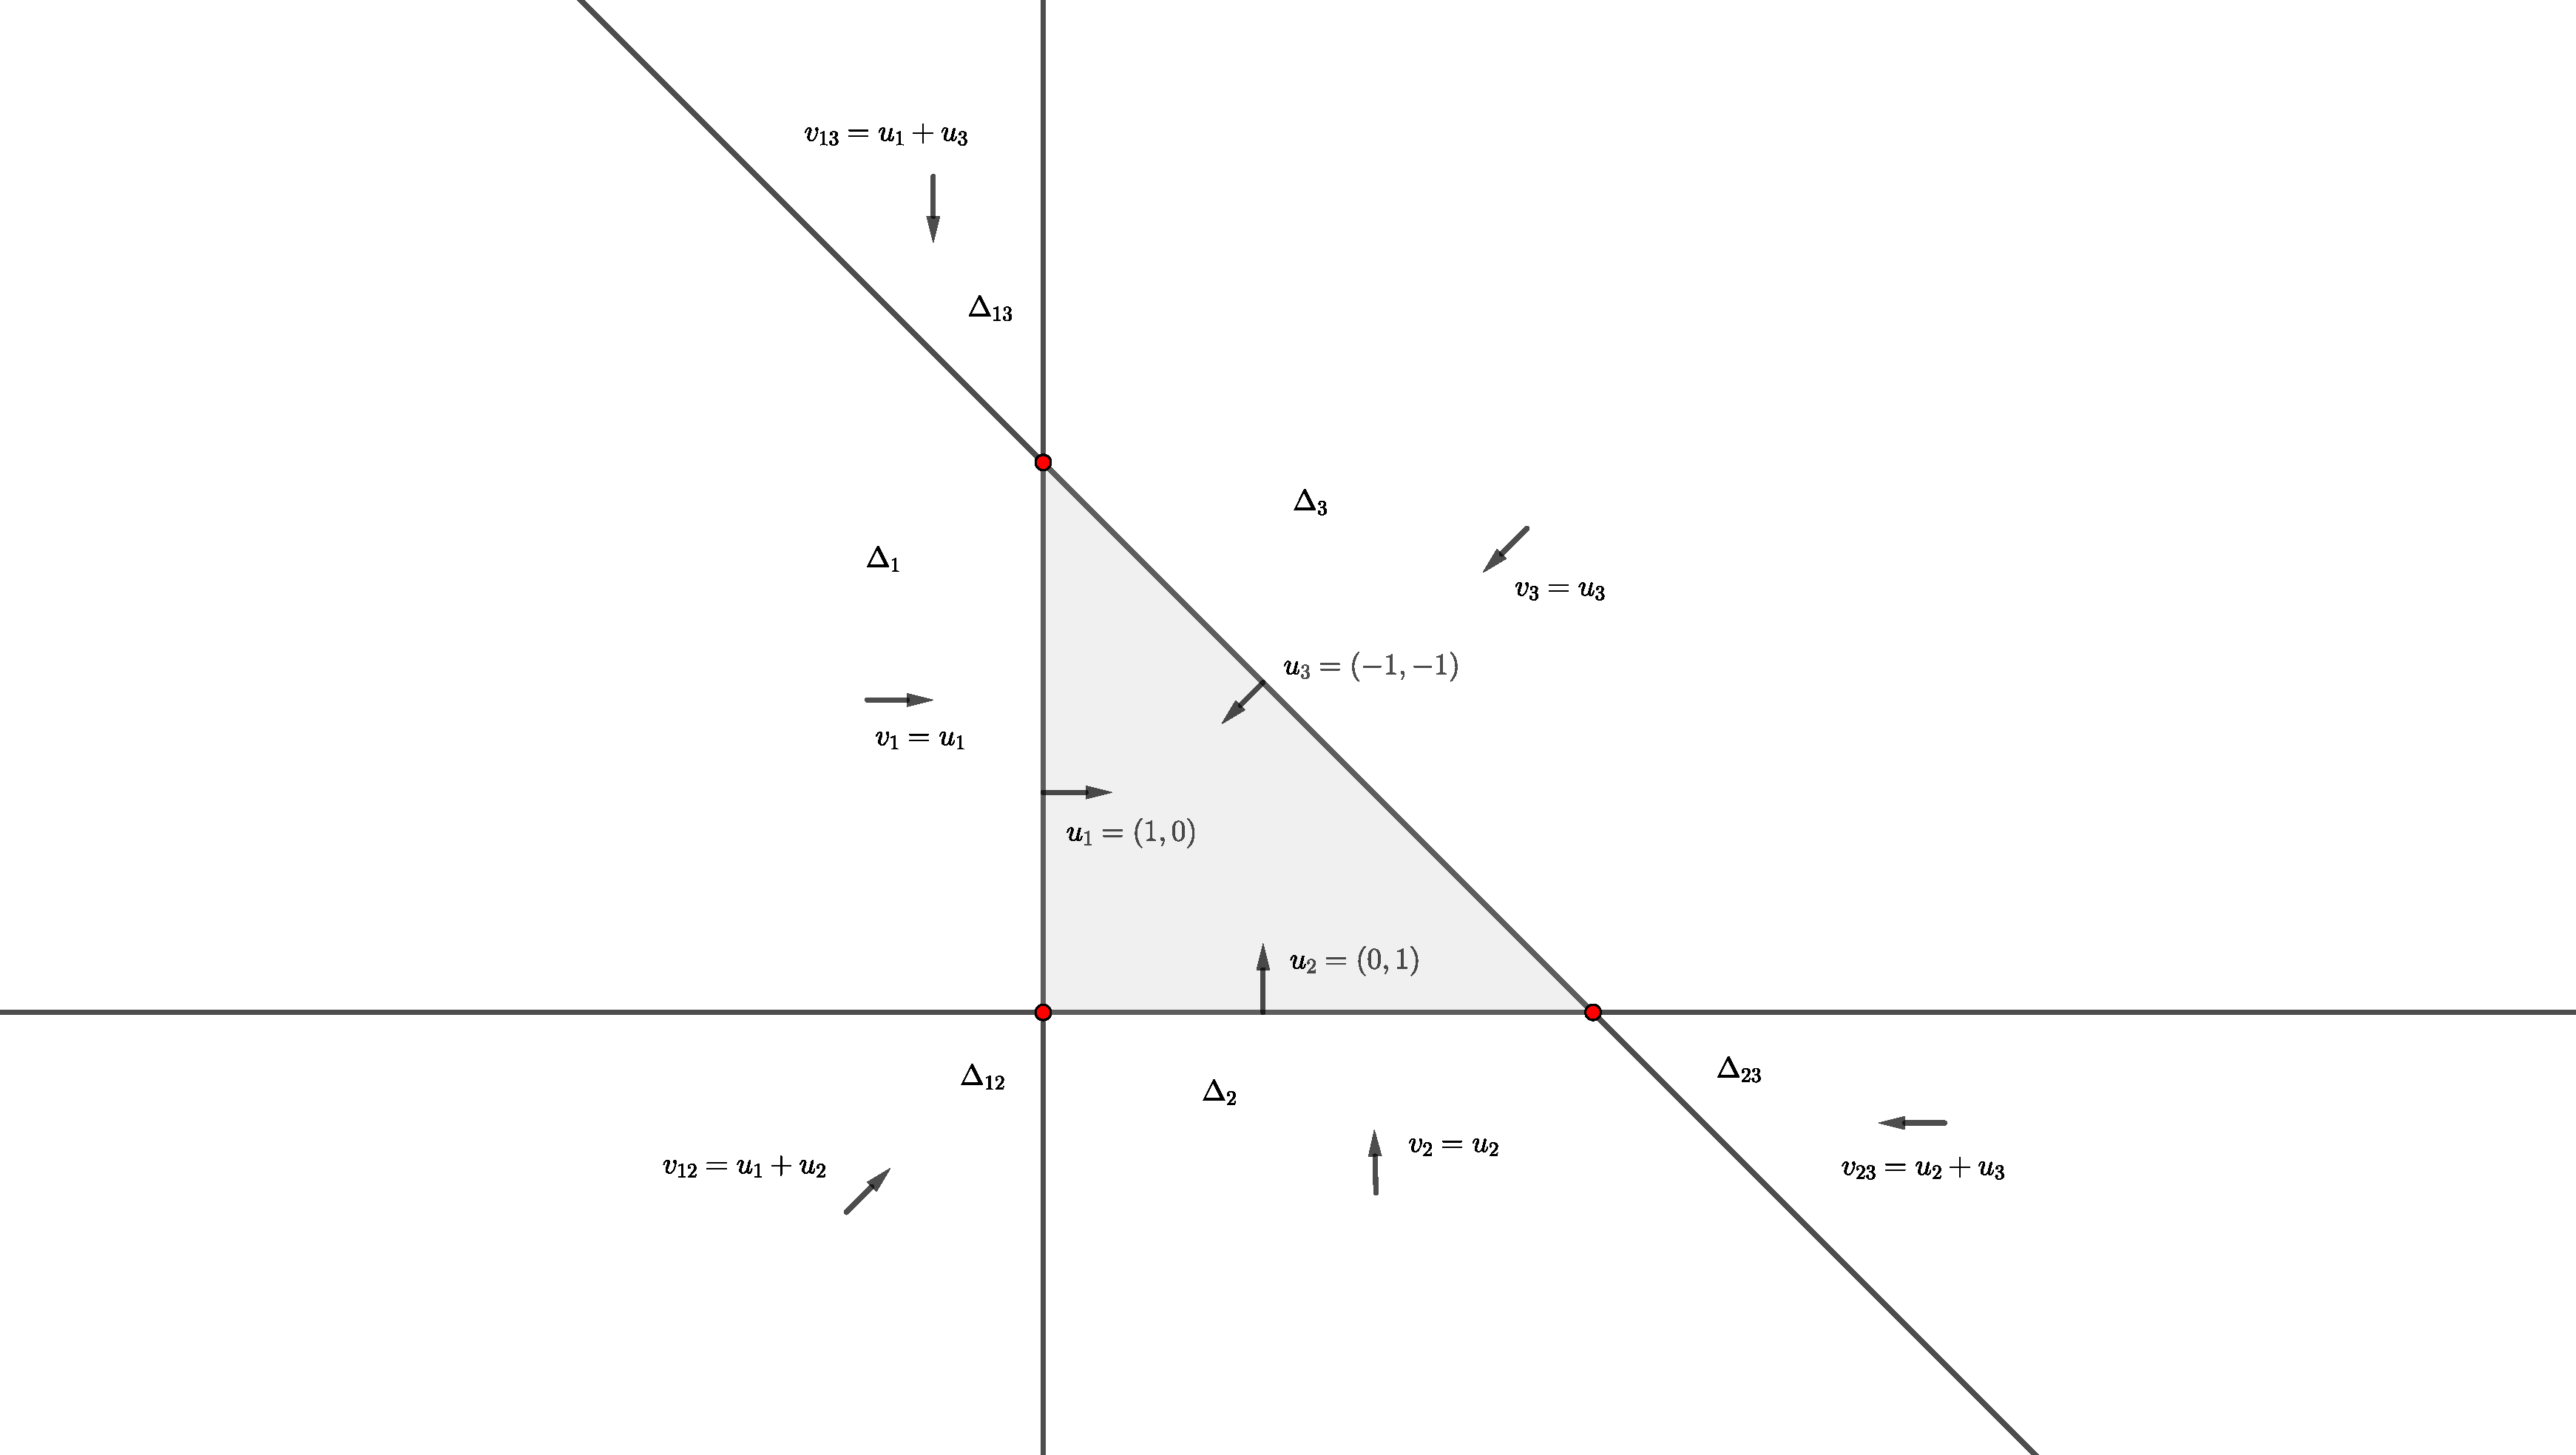
\includegraphics[width=1\linewidth]{figures/T_CP2_combinatorics.pdf}
			\caption{Combinatorics of the action of the residual $S^{1}$-action on the extended core $\mcE_{A}$ of $T^{\ast}\CC\PP^{2}$, represented by each generator $v_{A}$ of $S_{A}^{1}$ in $T^{2}$.}
%			\label{fig:test1}
		\end{figure}
		

	
	\end{example}

	\begin{example}
		For $\mf{M}$ whose core consists of two $\CC\PP^{2}$ intersecting at a point, so that the image of the real moment map is non-convex (todo)
		
		\begin{figure}[h!]
			%		\centering
			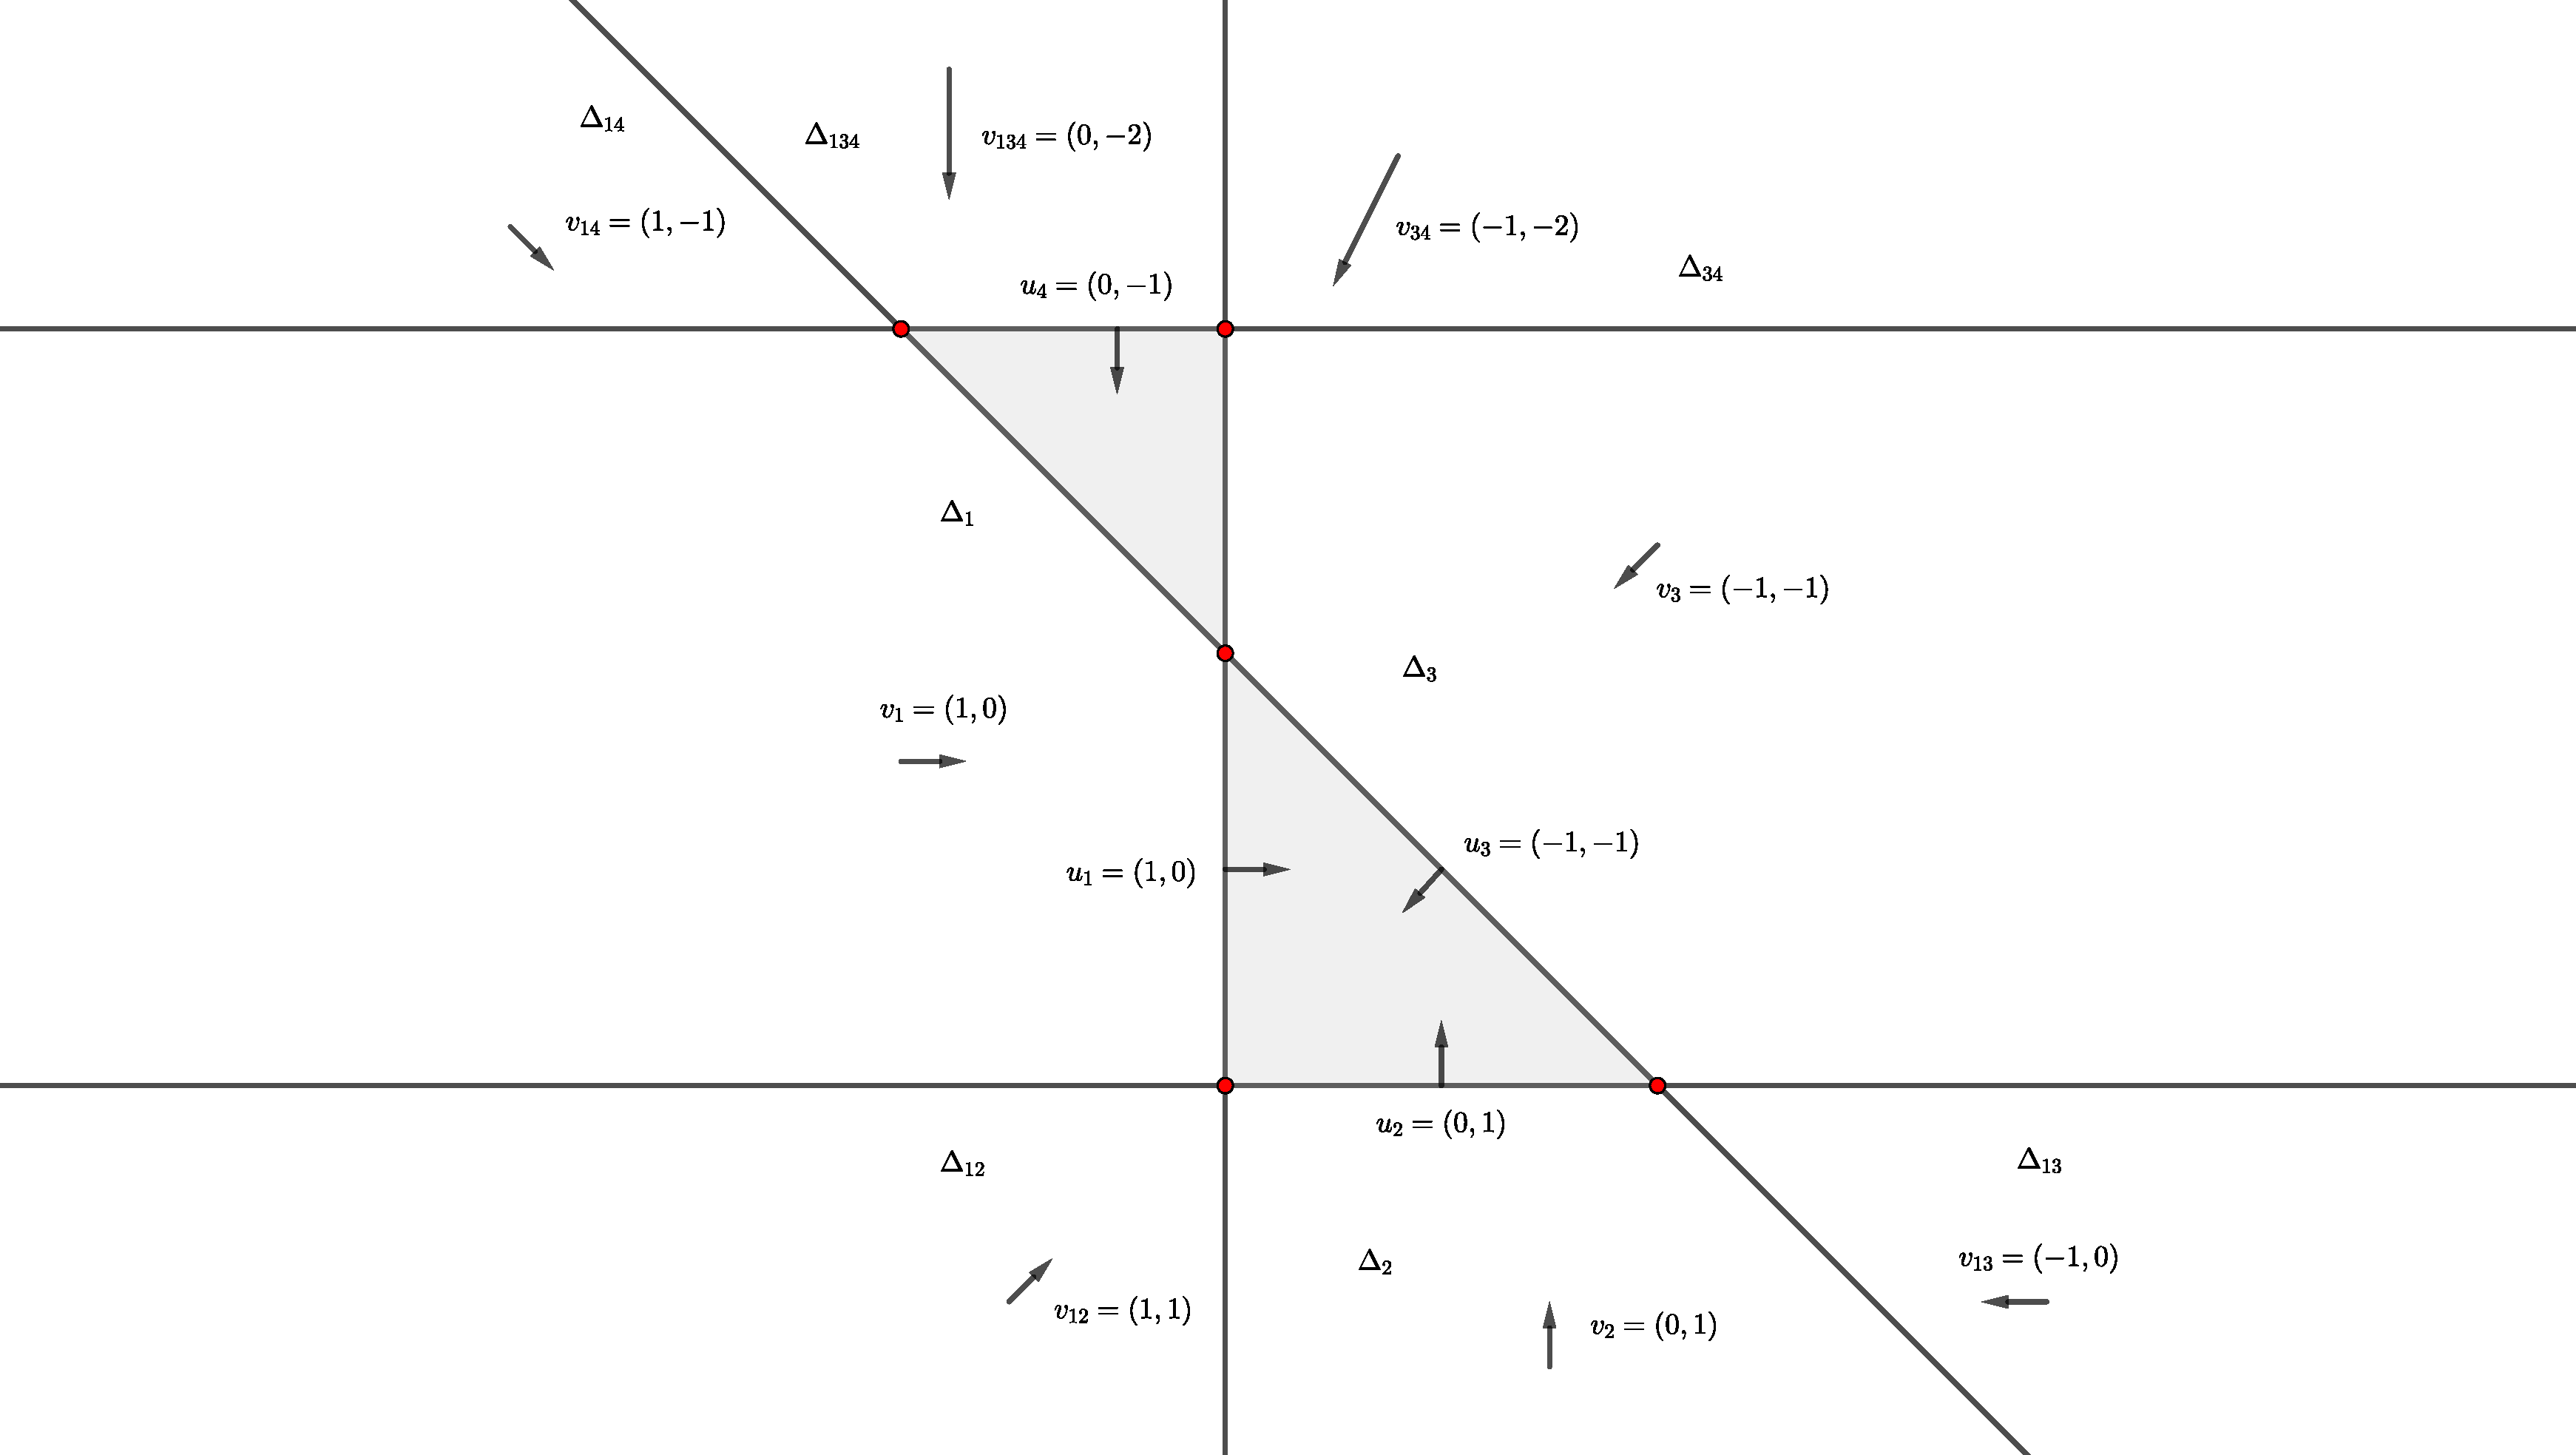
\includegraphics[width=1\linewidth]{figures/non-convex_combinatorics.pdf}
			\caption{Combinatorics of the action of the residual $S^{1}$-action when the core consists of two non-convex components.}
			%			\label{fig:test1}
		\end{figure}
		
		
		
	\end{example}
	
	\section{Compactifying the Hypertoric Variety via Symplectic Cutting}
	
	We will use the $S^{1}$-action to perform a symplectic cut of the toric \HK manifold $\mf{M}$ to compactify it, which has the effect of bounding the $\|w\|^{2}$ norm component of $\bar{\mu}_{\RR}$ by above, and discarding the rest that lies above this bound. Consider the product $\mf{M} \times \CC$,  and let $S^{1}$ act on $\mf{M} \times \CC$ via the diagonal product action, i.e. $S^{1}$ acts on $M$ by rotating the cotangent fibre coordinates, and on $\CC$ in the standard way:
	$$
	e^{i\theta} \cdot \big( [z,w], \xi   \big) = \left( e^{i\theta} \cdot [z,w], e^{i\theta}\xi\right) = \left( [z,e^{i\theta}w], e^{i\theta}\xi\right).
	$$
	This action is Hamiltonian, and the corresponding moment map $\Phi : \mf{M} \times \CC \ra \RR_{\geq 0}$ for the $S^{1}$-action is
	\[
		\Phi\big( [z,w], \xi  \big) = \phi[z,w] + |\xi|^{2} = \|w\|^{2} + |\xi|^{2}.
	\]
	Then we have
	\begin{equation*}
		\begin{split}
			\Phi^{-1}(\e) &= \big\{ ([z,w],\xi) \in M \times \CC \st \|w\|^{2} + |\xi|^{2} = \e    \big\} \\
			&= \big\{ [z,w] \in M \st \|w\|^{2} = \e    \big\} \bigsqcup \big\{ ([z,w],\xi) \in M \times \CC \st |\xi| = \pm\sqrt{\e - \|w\|^{2}} \big\} \\
			&= \big\{ [z,w] \in M \st \|w\|^{2} = \e    \big\} \bigsqcup \big\{ ([z,w],\xi) \in M \times \CC \st \xi = e^{i\arg(\xi)}\sqrt{\e - \|w\|^{2}}    \big\} \\
			&= \phi^{-1}(\e) \bigsqcup \lbracket \mf{M} \times S^{1}\rbracket \\
			&=: \Sigma_{1} \sqcup \Sigma_{2},
		\end{split}
	\end{equation*}
	where we denote the level-set $\phi^{-1}(\e) \subseteq \mf{M}$ by $\Sigma_{1}$, and $\Sigma_{2} \cong \mf{M} \times S^{1}$ is the trivial $S^{1}$-bundle over $\Sigma_{2}$ given by the globally defined section
	\begin{equation*}
		\mf{M} \rightarrow \mf{M} \times S^{1}, \qquad [z,w] \longmapsto \big( [z,w], e^{i\theta}\sqrt{\e - \|w\|^{2}}\big), \qquad e^{i\theta} \in S^{1}.
	\end{equation*}
	Finally, taking the symplectic reduction of $\Phi^{-1}(\e)$ with respect to the $S^{1}$-action, we obtain the \emph{symplectic cut of $\mf{M}$ at level-$\e$},
	\begin{equation*}
		M_{\leq \e} := \Phi^{-1}(\e)/S^{1} = \Sigma_{1}/S^{1} \bigsqcup \Sigma_{2}/S^{1},
	\end{equation*}
	where $\Sigma_{1}/S^{1} \cong \phi^{-1}(\e)/S^{1}$ is just the usual symplectic reduction, and where $\Sigma_{2}/S^{1}$ is diffeomorphic to $\mf{M}$ for $\|w\|^{2} < \e$, which we will denote by $\mf{M}_{<\epsilon}$.
	
	\subsection{The Combinatorics of the Cut Space, $\mf{M}_{\leq \e}$}
	
	Since the residual circle $S^{1}$-action acts as a subtorus $S_{A}^{1}$ of the residual torus $T^{d}$ on each component $\mc{E}_{A}$ of the extended core, the hyperplane arrangement determined in $(\mft^{d})^{\ast}$ by the real moment map $\bar{\mu}_{\RR}$ is compactified by dropping in half-spaces with an inwards-pointing normal vector, given by $v_{A}$ when taking the cut. 
	
	Recall from the previous section that $j_{A}: S_{1} \hookrightarrow T^{n}$ denoted the inclusion homomorphism of $S^{1}$ into the big torus $T^{n}$. If we let $j_{A, \ast}: \mf{s}^{1} \rightarrow \mft^{n}$ represent the differential of this inclusion, then
	\[
		j_{A,\ast}(1) = \sum_{i \in A} e_{i} \in \mft^{n},
	\]
	and the generator $\exp(v_{A})$ of the one-parameter subgroup $S_{A}^{1}$ in $T^{d}$ is
	\[
		\exp(v_{A}) = \exp\lbracket \pi_{\ast} \circ j_{A, \ast}(1) \rbracket,
	\]
	or to be more concise,
	\[
		S_{A}^{1} = \Set{ \exp \lbracket r \cdot \sum_{i \in A} u_{i} \rbracket | r \in \RR }.
	\]
	Then the moment map for this restriction for the $S^{1}$-action is
	\begin{equation*}
		\Phi[z,w] = j_{A}^{\ast} \circ \mrr[z,w] = \bigg\langle \mrr(z,w), \sum_{i\in A}\xi_{i} u_{i} \bigg\rangle,
	\end{equation*}
	and so from our above discussion of how we constructed the symplectic cut, the image in $(\RR^{d})^{\ast}$ of the symplectic quotient $\Phi^{-1}(\e)/S^{1}$ is
	\begin{equation*}
		\prr(\Phi^{-1}(\e)) = \bigg\{ y \in \Delta_{A} \st \bigg\langle y, \sum_{i\in A}\xi_{i}u_{i}\bigg\rangle + \e = 0 \bigg\} =: H_{A}
	\end{equation*}
	which introduces an inward-pointing half-space
	\begin{equation*}
		F_{A} := \bigg\{ y \in \Delta_{A} \st \bigg\langle y, \sum_{i\in A}\hbar_{i}u_{i}\bigg\rangle + \e \geq 0 \bigg\}
	\end{equation*}
	such that the image of the extended core component $\mc{E}_{A}$ after being compactified is the original convex polytope $\Delta_{A}$ intersected with $H_{A}$. One can also see clearly that the symplectic quotient $\Phi^{-1}(\e)/S^{1}$ has the restricted $S^{1}$-action as its stabiliser subgroup since, by definition of $H_{A}$, the moment map $\Phi|_{\mc{E}_{A}}$ equals the hyperplane $H_{A}$, \ie $\Phi|_{\mc{E}_{A}}$ is constant along $\Phi^{-1}(\epsilon)/S^{1}$.
	
	\begin{remark}
		If we had used instead the following action for $S^{1}$
		\begin{equation*}
			e^{i\theta}\cdot \big( [z,w], \xi \big) = \big( [z,e^{i\theta}w], e^{-i\theta}\xi \big)
		\end{equation*}
		with respective moment map
		\begin{equation*}
			\m_{\text{cut}} ([z,w],\xi) = \frac{1}{2}\|w\|^{2} - \frac{1}{2}|\xi|^{2} - \e,
		\end{equation*}
		and taken the cut, then the resulting then we would obtain the other ``discarded half'' $\mf{M}_{>\e}$ of the hypertoric manifold $\mf{M}$ along with the symplectic quotient $\Phi^{-1}(\e)/S^{1}$ with the opposite orientation:
		\begin{equation*}
			\mf{M}_{\geq \e} = \mf{M}_{> \e} \bigsqcup \Big(-(\Phi^{-1}(\e)/S^{1})\Big).
		\end{equation*}
		The component $M_{\e}$ is non-compact however, so we focus on $M_{<\e}$.
	\end{remark}
	
	The following two figures show the resulting moment polytope after compactification, for the hypertoric varieties $T^{\ast}\CC\PP^{2}$ and $T^{\ast}\CC\PP^{3}$.

	

	
	
	
	
	
	
	
	
	
	
	
	
	
	
	
	
	
	
	
	
	
	
	\bibliographystyle{unsrt}  
	\bibliography{preprint-01_bibliography}  %%% Remove comment to use the external .bib file (using bibtex).
	%%% and comment out the ``thebibliography'' section.
	
	%%% Comment out this section when you \bibliography{references} is enabled.
	
\end{document}
